\chapter{Come Bitcoin ottiene la Decentralizzazione}

Uno degli obiettivi primari di Bitcoin è la creazione di un \textbf{sistema di pagamento puramente distribuito e decentralizzato}. Tuttavia, implementare e mantenere una rete senza alcun punto centrale di controllo rappresenta una sfida ingegneristica e di teoria dei giochi estremamente complessa.

Esistono molti sistemi informatici che utilizzano architetture distribuite ma non completamente decentralizzate. Un esempio quotidiano è il sistema delle email (protocollo SMTP): pur non essendoci un unico server mondiale, il sistema è "federato", ovvero si appoggia a un numero ristretto di grandi provider (es. Google, Microsoft) che fungono da intermediari per gli utenti. Bitcoin, al contrario, ambisce a eliminare del tutto queste figure centrali.

\section{Le domande fondamentali del sistema}
Per comprendere come Bitcoin realizzi questa decentralizzazione, dobbiamo capire come il protocollo risponde a cinque domande cruciali che, nei sistemi tradizionali, vengono risolte da un Ente Centrale (come una Banca o uno Stato):
\begin{enumerate}
    \item \textbf{Gestione del registro:} Chi mantiene e aggiorna la copia ufficiale della blockchain?
    \item \textbf{Validazione:} Chi possiede l'autorità per stabilire quali transazioni sono valide e quali no?
    \item \textbf{Emissione:} Chi crea nuova moneta e secondo quali tempistiche?
    \item \textbf{Governance:} Chi determina le regole del protocollo e come vengono implementati gli aggiornamenti software?
    \item \textbf{Valore di scambio:} Come si determina il valore della moneta rispetto al mercato reale? \textit{(A differenza delle valute fiat, il protocollo Bitcoin non gestisce questo aspetto, lasciandolo interamente alle dinamiche di libero mercato, ovvero alla legge della domanda e dell'offerta sui vari exchange).}
\end{enumerate}

Oltre a questi interrogativi di sistema, vi sono questioni legate all'utente finale: come e dove conservare le proprie monete (i \textit{wallet} crittografici) e come interfacciarsi con la rete per effettuare le operazioni.

\section{I tre pilastri della decentralizzazione}
La risposta di Bitcoin a queste sfide si articola su tre livelli principali:
\begin{itemize}
    \item \textbf{Network Peer-to-Peer (P2P):} La rete non ha server centrali. Ogni nodo (computer) connesso è uguale agli altri, propaga le transazioni e mantiene una copia indipendente e verificata dell'intera blockchain.
    \item \textbf{Mining (Consenso e Creazione):} La validazione delle transazioni e la creazione di nuove monete avvengono tramite un processo competitivo noto come \textit{Proof of Work}. Chiunque può, in linea di principio, dedicare potenza di calcolo per partecipare alla sicurezza della rete.
    \item \textbf{Sviluppo e Aggiornamenti:} Il codice sorgente di Bitcoin è \textit{open-source}. Le modifiche al software vengono proposte pubblicamente e richiedono un ampio consenso da parte della rete (nodi e miner) per essere adottate.
\end{itemize}

\subsection*{Decentralizzazione: Teoria vs. Pratica}
È fondamentale sottolineare che il sistema è aperto a tutti \textit{sulla carta}, ma la realtà operativa attuale presenta delle sfumature. Ad esempio, il mining è teoricamente accessibile a chiunque possieda un computer; tuttavia, l'enorme competizione ha reso impossibile minare in solitaria in modo redditizio senza l'ausilio di hardware specializzato (ASIC) e senza unirsi a grandi \textit{Mining Pool} (cooperative di miner). Questo introduce, di fatto, un certo grado di "centralizzazione pratica" in un sistema nato per essere totalmente decentralizzato.

\section{Il Consenso Distribuito}

L'obiettivo principale della rete è fare in modo che tutti i nodi raggiungano un accordo condiviso (consenso) sullo stato del registro, stabilendo, ad esempio, quale debba essere il prossimo blocco da aggiungere alla catena.

Supponiamo che l'utente A voglia inviare un pagamento all'utente B. A si preoccuperà di trasmettere (in \textit{broadcast}) la transazione a tutti i nodi a cui è connesso. Questi la verificheranno e, se risulta valida, la manterranno in memoria pronti a inserirla in un blocco. 
Tuttavia, in un dato istante, non tutti i nodi hanno la stessa identica visione della rete: a causa dei fisiologici tempi di propagazione, i nodi potrebbero avere set di transazioni in sospeso leggermente diversi. Il consenso in Bitcoin, infatti, non è \textbf{immediato}, ma \textbf{emergente e a lungo termine}. I blocchi vengono proposti in media ogni 10 minuti, ma il consenso assoluto sull'irreversibilità di una transazione si consolida solo dopo circa un'ora (attendendo la conferma di almeno 6 blocchi successivi).

\subsection*{Le sfide del consenso: Latenza e Generali Bizantini}
Immaginiamo che tre nodi (es. rosso, blu e verde) propongano contemporaneamente il proprio set di operazioni valide sotto forma di blocco. La rete deve avere un meccanismo per sceglierne uno solo, che tutti gli altri dovranno poi verificare e accettare. Questo processo è ostacolato da diversi fattori del mondo reale:
\begin{itemize}
    \item Latenza e partizioni di rete (non tutti i nodi comunicano alla stessa velocità).
    \item Nodi che crashano o si disconnettono improvvisamente.
    \item \textbf{Nodi malevoli} che tentano di ingannare il sistema.
\end{itemize}

In informatica, la difficoltà di raggiungere un accordo in presenza di attori malevoli o fallaci è nota come il \textbf{Problema dei Generali Bizantini}. 

Per risolverlo, Bitcoin assume un modello in cui i nodi sono \textit{razionali}: essi seguono le regole del protocollo non per "bontà", ma perché il sistema di incentivi economici (la ricompensa in bitcoin) rende l'onestà molto più redditizia rispetto a un tentativo di attacco.

\subsection*{Il problema dell'identità: Sybil Attack}
Nei sistemi distribuiti classici o chiusi, il problema dei nodi malevoli si argina legando ogni nodo a un'identità reale e verificata (es. tramite un'autorità centrale). In Bitcoin, però, questo approccio non è applicabile: il sistema è progettato per garantire lo \textbf{pseudo-anonimato}, dove l'unica "identità" è rappresentata da una coppia di chiavi crittografiche.

Poiché chiunque può generare infinite chiavi a costo zero, la rete risulta esposta al \textbf{Sybil Attack}. In questo scenario, un singolo attaccante potrebbe creare migliaia di nodi fittizi per acquisire la maggioranza artificiale nella rete, sovrastare i nodi onesti e prendere il controllo delle decisioni.

Per neutralizzare il Sybil Attack e raggiungere il consenso senza fare affidamento su identità fisse, Bitcoin introduce un meccanismo innovativo. L'elezione del nodo che avrà il diritto di proporre il blocco successivo non avviene per votazione (dove i nodi fittizi vincerebbero), ma tramite una sorta di "lotteria" competitiva.
\subsection*{Algoritmo di Consenso}
Ad ogni round, viene estratto in maniera randomica un il leader temporaneo, che sceglie il blocco da aggiungere. Gli altri nodi della rete non possono influenzare l'estrazione, ma mantengono il potere di \textbf{validazione} e se il leader propone un blocco contenente operazioni non valide, il resto della rete lo ignorerà, rifiutandosi di estendere la blockchain a partire da quel blocco e, di fatto, creando una biforcazione. Tuttavia, poiché l'euristica per continuare una catena è quella di \textbf{continuare la catena più lunga}, quella biforcazione nata dall'inserimento di transazioni non valide morirà lì e nessuno la considererà valida. Questo meccanismo viene detto \textbf{Consenso implicito}.

Supponendo quindi di voler descrivere un algoritmo di consenso nella sua forma più semplice potremmo fare come segue:
\begin{enumerate}
    \item Le nuove transazioni vengono \textbf{inviate in broadcast} a tutta la rete.
    \item Ogni nodo le mette da parte e forma dei blocchi.
    \item Ad ogni round, viene scelto random un leader che propagherà il suo blocco a tutti gli altri nodi.
    \item Gli altri nodi controlleranno il blocco verificando che le transazioni sono valide e, nel caso in cui lo vogliano considerare valido, faranno la prossima aggiunta inserendo in testa a quel nodo.
\end{enumerate}

Analizziamo quindi cosa può e cosa non può cercare di fare un nodo malevolo:
\begin{itemize}
    \item \textbf{Può rubare Bitcoin?} Per quanto possa provarci, se le chiavi crittografiche di un utente sono state generate in maniera sicura, questo non potrà mai accadere poiché l'attaccante non riuscirebbe a generare una firma valida.
    \item \textbf{Denial of Service vs Bob?} Supponiamo che un nodo non voglia ammettere una certa transazione valida, questa potrebbe non venire mai scelta? Di fatto no poiché per quanto possa stare antipatico Bob, alcuni nodi onesti potrebbero comunque inserirla e, dunque, l'unico effetto sarebbe il delay della transazione. 
    \item \textbf{Double-Spending?} Immaginiamo questo scenario: A fa' una transazione verso B e ottiene (senza attendere) un certo bene. La transazione con il pagamento $A \to B$ viene salvata nel prossimo blocco della blockchain, tuttavia successivamente A diventa il leader e crea una fork con un altro pagamento $A \to C$. Poiché entrambe le fork sono valide, i nodi potrebbero scegliere arbitrariamente quale allungare (di solito si procede con il principio di allungare la catena più lunga). Così facendo A ha effettivamente fatto due pagamenti spendendo, però, una sola volta monete. 
    \begin{figure}[H]
        \centering
        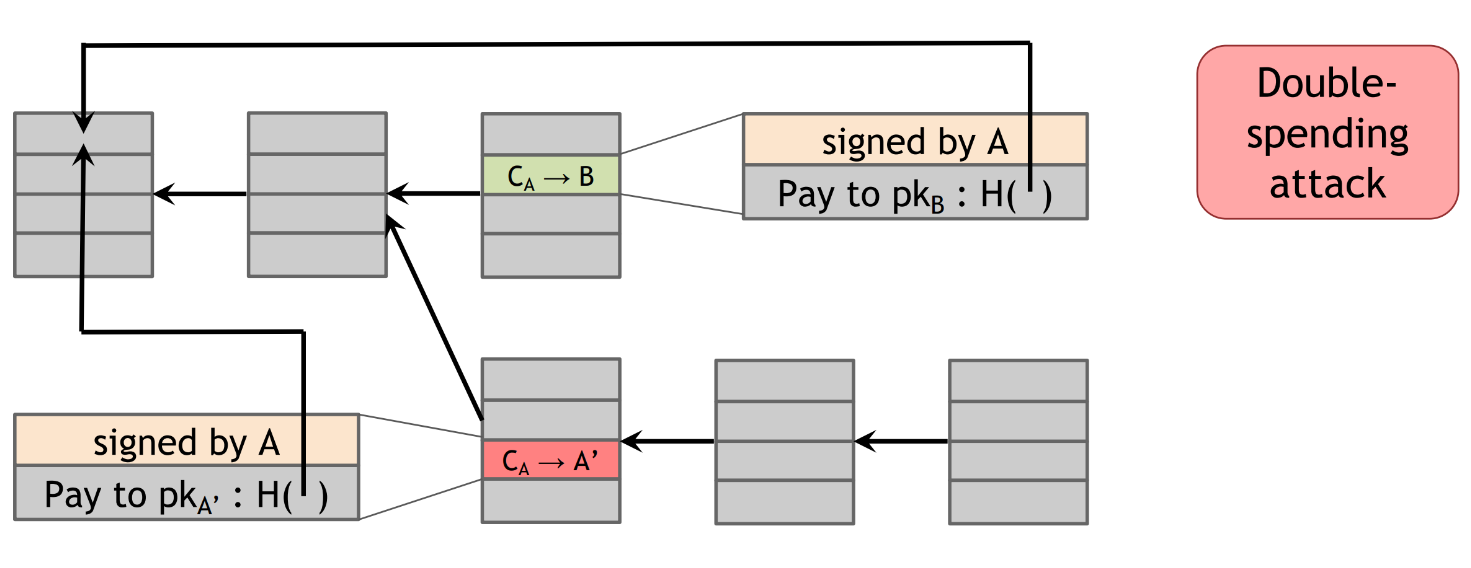
\includegraphics[width=0.7\linewidth]{Images/capitolo_2/double_spending_bc.png}
    \end{figure}
    Per evitare di questi problemi, è necessario che il blocco sia sufficientemente "in fondo" nella catena e, generalmente, lo consideriamo permanente dopo circa 6 blocchi successivi.
\end{itemize}
\subsection{Incentivi e Proof of Work}
Come abbiamo detto, assumeremo che tutti gli utenti della rete o quasi si comportino in maniera \textit{razionale}. Dunque, faremo sì di dare incentivi e penalità per far sì che questi si comportino secondo le regole. Innanzitutto abbiamo due incentivi per la partecipazione attiva all'allungamento della blockchain:
\begin{enumerate}
    \item \textbf{Block Reward: }Quando viene inserito un blocco nella catena, colui che lo ha proposto guadagna dei bitcoin tramite la \textit{coin create transaction}. Poiché i Bitcoin hanno un valore reale di mercato fare ciò conviene. Inoltre, scoraggiamo la creazione di blocchi non validi poiché questi non verrebbero considerati e, dunque, si "perderebbero" soldi. (parleremo tra poco di Proof of Work).
    \item \textbf{Transaction Fees: }Quando viene aggiunto un blocco, oltre che un guadagno dato dalla coin create transaction, coloro che mandano le transazioni aggiungono una mancia che viene guadagnata da colui che propone il blocco. Così facendo, si incentiva a mettere transazioni con più mancia all'interno della blockchain.
\end{enumerate}

Come possiamo facilmente intuire, è chiaro che il potere di aggiungere un nuovo blocco è qualcosa di molto ambito e che non possiamo effettuare tramite scelte casuali (anche perché come detto, saremmo soggetti a Sybil attack). L'idea diventa quindi non quella di scegliere un nodo del tutto a caso, bensì \textbf{scegliamo il prossimo nodo in base a quanto questo ha contribuito in termini di risorse allo sviluppo della rete}. Queste risorse devono essere non monopolizzabili e non duplicabili. Questo può essere effettuato tramite \textbf{Proof of Work} cioè quanta potenza computazionale si è data alla rete e tramite \textbf{Proof of Stake} cioè si sceglie in base a quanto è disposto a "spendere" un nodo per aggiungere il prossimo blocco. Questi sono rispettivamente adottati in Bitcoin ed Ethereum. 

\subsection*{Hash Puzzle}
Per quanto riguarda nello specifico Bitcoin, abbiamo la Proof of Work che è \textbf{l'hash puzzle}. In pratica quello che facciamo è creare il blocco includendo tutte le transazioni e l'hash pointer precedente e cercando una nonce tale che è l'intero Hash del blocco abbia una serie di zero all'inizio. Maggiori saranno gli zeri da cercare, più sarà difficile procurarsi quest'hash e, se la funzione hash è sicura, allora l'unico modo per trovare questa nonce è essere fortunati o provare tantissime combinazioni di Nonce.
Come dicevamo, quindi, colui che cerca l'hash mette potenza computazionale a disposizione e fare questo ha un certo costo anche in termini di elettricità. Dunque, fare questo sforzo per inserire transazioni non valide è chiaramente uno spreco di soldi. 
Inoltre, l'hash puzzle gode di due proprietà principali:
\begin{enumerate}
    \item \textbf{Difficile da calcolare: }come detto è necessaria una grande quantità di prove per trovare la giusta Nonce.
    \item \textbf{Parametrizzabile:} è facile regolare la difficoltà della ricerca fixando il numero di zeri da trovare. Questo viene fatto poiché vogliamo far sì che venga aggiunto un blocco all'incirca ogni 10 minuti.
    \item \textbf{Veloce da verificare: }Nonostante sia molto difficile da calcolare, resta il fatto che, una volta fornita la Nonce, questo sia estremamente facile da calcolare.
\end{enumerate}

Nell'intestazione del blocco Bitcoin, lo spazio dedicato alla Nonce standard è di soli \textbf{32 bit}. Questo significa che esistono "solo" circa $4,3$ miliardi di combinazioni, un numero che i moderni hardware esauriscono in frazioni di secondo senza trovare un hash valido. 
Per ovviare a questo problema, i miner sfruttano l'\textbf{extraNonce}, un campo inserito all'interno della transazione di ricompensa (\textit{Coinbase Transaction}). Modificando l'extraNonce, cambia l'hash di quella specifica transazione, generando un effetto a cascata che modifica l'intero Merkle Tree e aggiorna la \textbf{Merkle Root} nell'header. Questa piccola modifica fornisce al miner una base di partenza completamente nuova, permettendogli di testare altri 4,3 miliardi di combinazioni di Nonce.

\subsection*{Sostenibilità e Difficoltà Dinamica}
Perché la struttura sia sostenibile, deve garantire ai \textit{miner} un guadagno (Block Reward + Transaction Fees) mediamente superiore ai costi operativi (hardware ed elettricità). Se questo profitto non fosse possibile, i miner spegnerebbero i loro macchinari, compromettendo la sicurezza della blockchain. 

Tuttavia, il protocollo non garantisce un profitto fisso, poiché il valore della moneta fluttua sul mercato. Per compensare l'ingresso o l'uscita dei miner dalla rete, il protocollo regola automaticamente la \textbf{difficoltà dell'hash puzzle}. Questo aggiustamento non serve a salvaguardare i profitti, ma a garantire che, indipendentemente da quanta potenza computazionale sia attiva, venga scoperto un nuovo blocco in media \textbf{ogni 10 minuti}. Se molti miner entrano attratti dai profitti, la difficoltà si alza; se il prezzo crolla e molti miner spengono le macchine per non andare in perdita, la difficoltà si abbassa, permettendo alla rete di continuare a funzionare regolarmente.

\subsection*{L'Attacco del 51\%}
Come abbiamo visto, l'algoritmo di consenso funziona fintanto che la maggioranza della potenza computazionale (hash power) è in mano a nodi onesti. Ma cosa accadrebbe se un singolo attaccante (o un cartello di miner) riuscisse a controllare il \textbf{51\% dell'hash power} totale della rete? Analizziamo i vari scenari:

\begin{itemize}
    \item \textbf{Può rubare le monete di altri utenti?} No. Per autorizzare una transazione e spendere fondi altrui è necessaria la firma digitale creata con la chiave privata del legittimo proprietario. Nessuna potenza di calcolo (salvo i futuri computer quantistici) può falsificare questa firma.
    
    \item \textbf{Può cambiare il reward del blocco (creare monete dal nulla)?} No. Anche se il miner al 51\% creasse un blocco assegnandosi 1000 BTC di ricompensa invece di quelli previsti dal protocollo, gli altri nodi (i full node che verificano le regole) scarterebbero immediatamente il blocco considerandolo non valido, indipendentemente da quanta potenza di calcolo lo abbia generato.
    
    \item \textbf{Può sopprimere (censurare) del tutto le transazioni?} \textbf{Nella pratica, no.} Teoricamente, se un attaccante riuscisse a mantenere la maggioranza assoluta dell'hash power per sempre, potrebbe ignorare sistematicamente i blocchi onesti contenenti la transazione sgradita, costringendo la rete ad adottare la sua catena (più lunga e priva della transazione). 
    Tuttavia, la transazione non svanisce: rimane in attesa nella \textit{mempool} di tutti i nodi onesti. Poiché mantenere il 51\% dell'hash power comporta un costo energetico ed economico insostenibile nel lungo periodo, l'attaccante è destinato a perdere la maggioranza. Non appena ciò accade (o in momenti di forte varianza probabilistica in cui i miner onesti trovano più blocchi di fila), la rete onesta includerà la transazione. Inoltre, una censura palese e sistematica spingerebbe il \textit{social consensus} della rete ad attuare un \textit{Hard Fork} difensivo per neutralizzare l'hardware dell'attaccante, rendendo di fatto impossibile una censura definitiva.
    \item \textbf{Può distruggere la fiducia in Bitcoin (Double Spending)?} \textbf{Sì.} Il danno più grave di un attacco al 51\% è la possibilità di effettuare \textit{double spending} riscrivendo la storia recente della blockchain. L'attaccante può inviare dei fondi a un exchange, farsi convertire i BTC in dollari, e contemporaneamente minare in segreto una catena alternativa in cui invia quegli stessi BTC a un altro suo indirizzo. Avendo il 51\%, la sua catena segreta diventerà presto la più lunga; una volta pubblicata, la rete cancellerà la transazione verso l'exchange, permettendo all'attaccante di riprendersi i fondi.
\end{itemize}

\textbf{Perché non accade spesso?} 
Oltre all'enorme difficoltà logistica e all'altissimo costo per procurarsi l'hardware e l'energia necessari per un simile attacco, vi è un fortissimo \textbf{disincentivo economico}. Se un attacco del genere avesse successo su scala visibile, la fiducia nel network crollerebbe istantaneamente. Il valore di Bitcoin precipiterebbe, rendendo di fatto inutile il bottino rubato dall'attaccante e distruggendo l'enorme investimento milionario fatto per ottenere il 51\% dell'hardware.

\section{Struttura delle Transazioni e Modello UTXO}

Andiamo ora ad analizzare nel dettaglio come vengono strutturate ed effettuate le transazioni all'interno della blockchain. 

Uno dei problemi principali in un sistema finanziario decentralizzato è la verifica della disponibilità dei fondi: i nodi devono accertarsi che chi sta inviando del denaro ne sia effettivamente in possesso. Se adottassimo un approccio "ingenuo" (\textit{naive ledger}), in cui il registro tiene semplicemente traccia dei trasferimenti $A \to B$, per verificare il saldo di un utente saremmo costretti a ricalcolare l'intero storico delle sue transazioni partendo dal \textit{Genesis Block} (il primo blocco della catena). Questo causerebbe un dispendio di tempo e risorse computazionali insostenibile.

\begin{figure}[H]
    \centering
    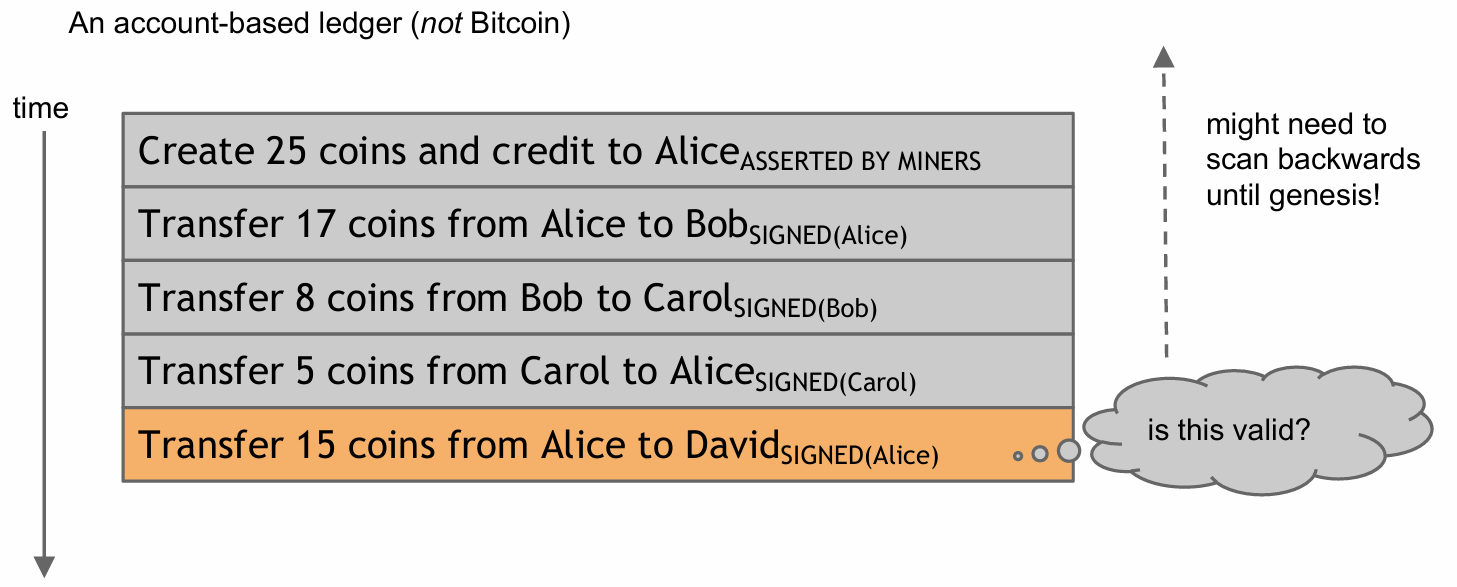
\includegraphics[width=0.7\linewidth]{Images/capitolo_2/account_ledger.png}
\end{figure}

Per risolvere questo problema con la massima efficienza, Bitcoin non utilizza il concetto di "conto bancario" con un saldo aggiornabile, ma sfrutta il \textbf{Modello UTXO (Unspent Transaction Output)}. 

In questo modello, le monete non esistono come saldi in un database, ma come "pezzi di metallo" digitali indivisibili (gli UTXO, appunto). Una transazione non fa altro che prendere in input dei vecchi UTXO, distruggerli, e creare in output dei nuovi UTXO.
\begin{figure}[H]
    \centering
    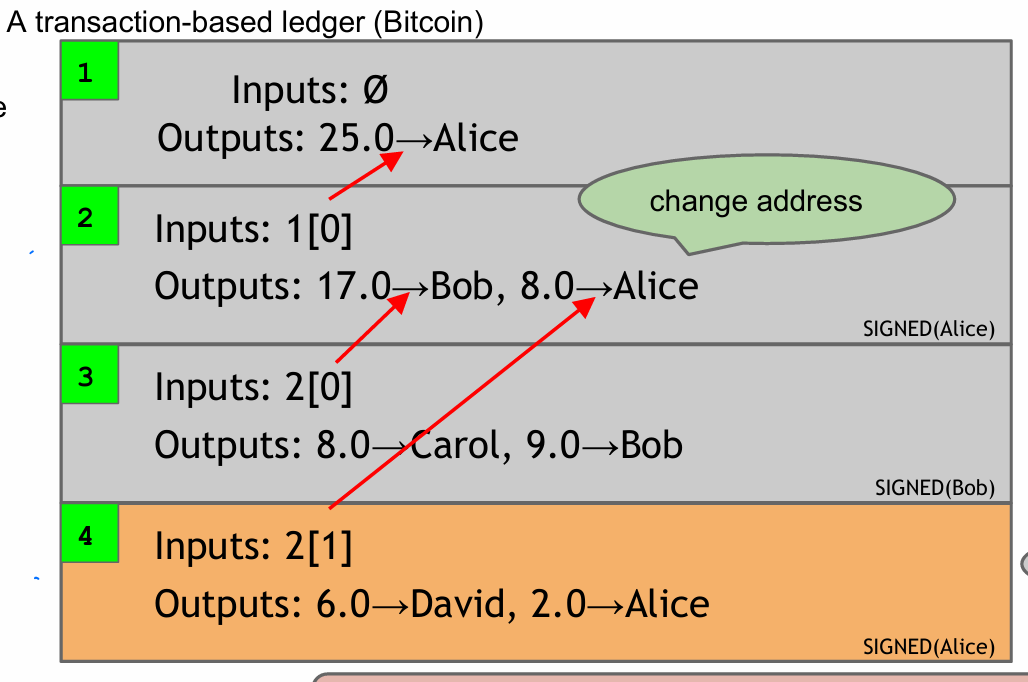
\includegraphics[width=0.7\linewidth]{Images/capitolo_2/input_out.png}
\end{figure}

Più nello specifico, una transazione è composta da:
\begin{itemize}
    \item \textbf{Input:} Per giustificare e finanziare la spesa, la transazione deve fornire degli \textit{hash pointer}. Questi puntatori indicano in modo univoco l'ID di una transazione precedente e l'indice specifico dell'output che si vuole spendere. Per poter usare questo input, l'utente deve fornire la firma digitale corrispondente (dimostrando di possedere la chiave privata di quell'indirizzo).
    \item \textbf{Output:} Definiscono i nuovi destinatari e i relativi importi. Poiché gli input (gli UTXO) \textbf{devono essere spesi per intero}, se il valore totale degli input è maggiore di quanto si vuole pagare al destinatario, la transazione dovrà generare un secondo output destinato al mittente stesso. Questo output aggiuntivo rappresenta il \textbf{resto} dell'operazione.
\end{itemize}

Grazie a questa struttura logica modulare, è possibile effettuare operazioni complesse con estrema facilità. Ad esempio, si possono realizzare \textbf{pagamenti congiunti} inserendo input provenienti da indirizzi diversi (per sommare i fondi); naturalmente, in questo caso, la transazione dovrà contenere una firma digitale separata e valida per ogni singolo input fornito. Inoltre, è anche possibile effettuare operazioni di \textbf{consolidamento} in cui si prendono in input più UTXO in proprio possesso per compattarli in un solo UTXO.

